
% Created 2011-10-27 do 16:51
\documentclass[a4paper, 11pt]{article}
\usepackage[utf8]{inputenc}
\usepackage[T1]{fontenc}
\usepackage{fixltx2e}
\usepackage{graphicx}
\usepackage{longtable}
\usepackage{float}
\usepackage{wrapfig}
\usepackage{soul}
\usepackage{textcomp}
\usepackage{tikz}
\usepackage{listings}
\usepackage{color}
\usetikzlibrary{positioning,shapes,shadows,arrows}
%\usepackage{marvosym}
%\usepackage{wasysym}
%\usepackage{latexsym}
\usepackage{amssymb}
\usepackage{mathtools}
\usepackage{hyperref}
\usepackage{placeins}
\usepackage{pict2e}
\usepackage{subfig}
\usepackage{appendix}
%\usepackage{cmbright}
\usepackage[english]{babel}
\usepackage[a4paper,margin=2.5cm]{geometry}
 \hyphenpenalty=5000
\tolerance=1000
\providecommand{\alert}[1]{\textbf{#1}}
\newfloat{MATLAB code}{h}{}
\usepackage{tikz,pgfplots}
\newcommand{\code}[1]{\textbf{\texttt{#1}}}
\pgfplotsset{compat=newest}
\pgfplotsset{plot coordinates/math parser=false}

\newcommand{\NAAM}{Roel Matthysen}
\newcommand{\RICHTING}{Master WIT Fase 1}
\newcommand{\SNUMMER}{s0202264}
%\newcommand{\NAAMT}{Nico Vervliet} 
%\newcommand{\RICHTINGT}{Master WIT Fase 1}
%\newcommand{\SNUMMERT}{s0203233}
\newcommand{\TITEL}{Nonlinear Systems}
\newcommand{\SUBTITEL}{Report on the exercise sessions}
\newcommand{\VAK}{Nonlinear Systems}
\newcommand{\PROFESSOR}{Prof. J. Suykens}
\newcommand{\PROFESSORb}{Prof. D. Roose}
\newcommand{\TAV}{}
\newcommand{\DATUM}{\today}


\newlength\figureheight
\newlength\figurewidth
\setlength\figureheight{2cm}
\setlength\figurewidth{12cm}


\begin{document}


\vspace*{-1cm}\hspace*{-1cm}
\begin{minipage}{0.5\textwidth}
\textsc{Faculteit}\\ \textsc{Ingenieurswetenschappen}\\
\end{minipage}\hfill%
\begin{minipage}{0.2\textwidth}
 \begin{flushright}
 
\includegraphics[width=2cm]{img/sedes2.pdf}
 \setlength{\unitlength}{1mm}
 \begin{picture}(28.5,2)
  \put(0,0){\line(1,0){28.5}}
 \end{picture}
 KATHOLIEKE\\UNIVERSITEIT\\LEUVEN
 \end{flushright}
\end{minipage}


\vfill
\pagestyle{empty}

\begin{center}
\begin{Huge}
\text{\TITEL}\\[4mm]
\end{Huge}
\begin{LARGE}
  \text{\SUBTITEL}
\end{LARGE}
\end{center}
\vfill
\begin{tabular}{p{0.59\textwidth}p{0.7\textwidth}}
   & \begin{Large}\textbf{\NAAM}\end{Large}\\
%  & \begin{Large}\textbf{\NAAMb}\end{Large}\\
   & \SNUMMER \\
   & \RICHTING\\
   & \\
%& \begin{Large}\textbf{\NAAMT}\end{Large}\\
%%  & \begin{Large}\textbf{\NAAMb}\end{Large}\\
%   & \SNUMMERT \\
%   & \RICHTINGT\\
%   & \\
   & \begin{large}\VAK\end{large}\\
   & \begin{large}\PROFESSOR\end{large}\\
   & \begin{large}\PROFESSORb\end{large}\\
   & % \begin{large}t.a.v.: \TAV\end{large}\\
%  & \hspace{4mm}\begin{large}\PROMOTORb\end{large}\\
\end{tabular}
\\
\\
\\ 
\begin{center}
\DATUM
\end{center}

\clearpage
\pagestyle{plain}


%%% Local Variables: 
%%% mode: latex
%%% TeX-master: "main"
%%% End: 

\tableofcontents
\clearpage

\section{Bead on a tilted wire}
\numberwithin{figure}{section}
In this section a bead with mass $m$ moves along a wire. As depicted in figure  \ref{fig:ex1beadeps}, the wire is rotated with an angle $\theta$ with respect to the vertical axis. The bead is connected to the bottom of the structure through a spring with spring constant $k$ and rest length $L_0$. The bead is also subject to a friction force $b\dot{x}$. 

\begin{figure}[htp]
\centering
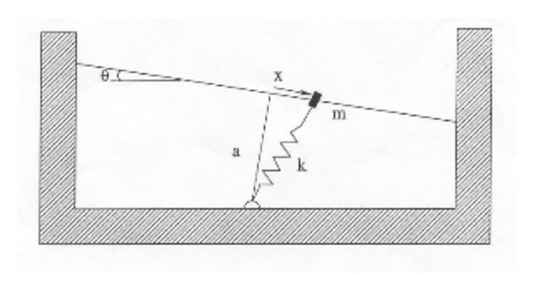
\includegraphics{img/ex1/bead.eps}
\caption{}
\label{fig:ex1beadeps}
\end{figure}

The system model represents Newton's equation for the motion of the bead on the wire
\begin{equation}
m\ddot{x}=mg\sin{\theta} -b\dot{x}-kx\left(1-\frac{L_0}{\sqrt{x^2+a^2}}\right)\label{eqn:newton2order}
\end{equation}
This system can be split up into a more useful form with variables $x$ and $\dot{x}$ and only first order derivatives
 \begin{align}
 \frac{dx}{dt}&=\dot{x}\label{eqn:dxdt}\\
 \frac{d\dot{x}}{dt}&=g\sin{\theta}-\frac{b}{m}\dot{x}-\frac{kx}{m}\left(1-\frac{L_0}{\sqrt{x^2+a^2}}\right)\label{eqn:ddotdt}
 \end{align}
 
 %% Theta=0
 
\subsection{The case $\theta=0$}\label{sec:ex1theta0}
In this section the system will be studied while the wire is vertical. This leads to a perfectly symmetrical system in $x$. 
\subsubsection{Fixed points and their stability}
In order to find the fixed points, a simple reasoning suffices. For the system of equations (\ref{eqn:dxdt})-(\ref{eqn:ddotdt}) to have a stationary solution at a point, both derivatives must be zero. From equation (\ref{eqn:dxdt}) it is clear that $\dot{x}$ must allways be zero. When this result is used in (\ref{eqn:ddotdt}), a condition on $x$ for $(x,0)$ to be a fixed point is obtained
\begin{align}
  \frac{d\dot{x}}{dt}=0&=-\frac{kx}{m}\left(1-\frac{L_0}{\sqrt{x^2+a^2}}\right)\label{eqn:ddotdt}
\end{align}
Thus either 
\begin{equation}
x=0 \mbox{\hspace{12pt}or\hspace{12pt}}x=\pm\sqrt{L_0^2-a^2}
\end{equation}
As is obvious from the formula, the two square roots will only exist if $a<L_0$. The stability of these fixed points can easily be derived when $m=0$. Equation\label{eqn:newton2order} then simplifies to the first order system
\begin{equation}
b\dot{x}=-kx\left(1-\frac{L_0}{\sqrt{x^2+a^2}}\right)\label{eqn:ex1firstorder}
\end{equation}
This derivative is plotted in figure \ref{fig:ex1stab} for both $a<L_0$ and $a>L_0$. From this figure it is clear that when $a<L_0$, the fixed points corresponding to the square roots are stable and the origin is unstable, and when $a>L_0$, the origin is stable. This is the typical behavior of a pitchfork bifurcation, as is shown in the bifurcation diagram in figure \ref{fig:ex1bif1}. The bifurcation diagram has free parameter $L_0$ and the pitchfork bifurcation occurs when $L_0=a$.
\begin{figure}[htp]
\centering
\subfloat[$a<L_0$]{
\includegraphics{img/ex1/stab1.eps}} \hspace{18pt}
\subfloat[$a>L_0$]{
\includegraphics{img/ex1/stab2.eps}}
\caption{}
\label{fig:ex1stab}
\end{figure}
\begin{figure}[htp]
\centering

\includegraphics{img/ex1/bif1.eps}
\caption{}
\label{fig:ex1bif1}
\end{figure}

The stability analysis is only valid when $m=0$. In order to determine for which relative values of $m$ this is a valid approximation, the system is first made dimensionless
\begin{equation}
\frac{m\ddot{x}}{ak}= -\frac{b\dot{x}}{ak}-\frac{x}{a}\left(1-\frac{L_0}{\sqrt{x^2+a^2}}\right)
\end{equation}
From this equation it is clear that the inertia term can only be neglected with respect to the other terms when $m<<b$, when the inertia is very small relative to the friction force.
\subsubsection{Comparison of the full system with its first order approximation}
For ease of use, the system is transformed to a simpler form
\begin{align}
\frac{\delta u}{\delta \tau} &= v \\
\frac{\delta v}{\delta \tau} &= -\frac{1}{\epsilon} [v+(1-\frac{R}{\sqrt{1+u^2}})u]
\end{align}
with 
\begin{equation}\label{eqn:ex1transfers}
R=\frac{L_0}{a}, u=\frac{x(t)}{a},v=\frac{\alpha \dot{x}(t)}{a},\epsilon=\frac{km}{b^2},\tau=\frac{t}{\alpha}\mbox{\hspace{4pt}and\hspace{4pt}} \alpha=\frac{b}{k}
\end{equation} 
When neglecting the inertia term as in (\ref{eqn:ex1firstorder}), a simplified first order system is obtained
\begin{equation}
\frac{\delta u}{\delta \tau}=(1-\frac{R}{\sqrt{1+u^2}})u
\end{equation}
The behavior of this first order approximation will be compared with the full system for $R=0.6463$. For this value of $R$ only the origin is stable. The parameter $\epsilon$ is varied for different starting values, and the two systems are then simulated until this equilibrium sets in. The results are shown in figure \ref{fig:ex1epsilon}. The bold curves are from the simulated first order system. The curves for the full system are shown for $\epsilon \in [0,0.5,1,2]$. As is obvious from the model equations, the two systems are equal when $\epsilon=0$. When $\epsilon$ grows, the behavior of the full system will distantiate from that of the first order approximation. The stable equilibrium is still reached, but the system has an overshoot that is not possible in first order systems.
\begin{figure}[htp]
\centering

\includegraphics{img/ex1/epsilon.eps}
\caption{}
\label{fig:ex1epsilon}
\end{figure}

A problem that is not yet considered is that of the initial value. For the full system, an initial position and velocity are required. In figure \ref{fig:ex1epsilon} this initial velocity is taken to be zero. However, the initial velocity of the first order system is determined by the equations. The initial velocity of the full system can be chosen according to this first order system. The results are shown in figure \ref{fig:epsilon2}. The solutions now start with the same velocity and their behavior is comparable for the first second, but aftwerwards the overshoot shows again and the solutions start to distantiate for growing $\epsilon$.
\begin{figure}[H]
\centering

\includegraphics{img/ex1/epsilon2.eps}
\caption{}
\label{fig:epsilon2}
\end{figure}

%% The case theta !=0
\subsection{The case $\theta \ne 0$}\label{sec:ex1thetane0}
The equations from section \ref{sec:ex1theta0} now gain a term depending on $\sin{\theta}$. When keeping the change of variables of (\ref{eqn:ex1transfers}) and adding $h=mg\sin{\theta}/ak$, the equilibrium equation becomes
\begin{equation}\label{eqn:ex1eqbreq}
1-\frac{h}{u}=\frac{R}{\sqrt{1+u^2}}
\end{equation}
which is equal to the equilibrium equation for $\theta=0$ except for the term in $h$. A graphical interpretation is given in figure \ref{fig:graphR}. In this figure $uR/\sqrt{1+u^2}-u+h$ is plotted as a function of $u$ for $h=0$ (bold curve) and $h=\pm0.1$ (striped curves). Where the graph intersects the x-axis an equilibrium is found. When interpreting the equilibrium equation in this way, it is seen that the parameter $h$ only shifts the curve along the $y$-axis. When $R<1$, the curve is monotonic and the parameter $h$ will only affect the position of the equilibrium, which is always stable. When $R>1$ there are three possibilities
\begin{itemize}
\item $|h|>h_c$, as in the striped curves. There is only one intersection with the x-axis, and thus only one (stable) equilibrium.
\item $|h|=h_c$, as in the red striped curve. At this point the curve's local minimum or maximum will touch the x-axis, and a pair of stable and unstable fixed points appears or disappears in a saddle-node bifurcation.
\item $|h|<h_c$, as in the bold curve. The curve intersects the x-axis at three different points. Two of the equilibria are stable, the one in the middle is unstable.
\end{itemize}
\begin{figure}[H]
\centering
\subfloat[$R<1$]{
\includegraphics{img/ex1/graphR1.eps}}\hspace{18pt}
\subfloat[$R>1$]{
\includegraphics{img/ex1/graphR2.eps}\label{fig:graphR2}}
\caption{}
\label{fig:graphR}
\end{figure}
When replacing $R$ by $r+1$ in the equilibrium equation (\ref{eqn:ex1eqbreq}), the equation can be simplified for small $r$, $h$ and $u$
\begin{align}
1-\frac{h}{u}&=\frac{r+1}{\sqrt{1+u^2}} \\
(u-h)\sqrt{1+u^2}&=ur+u \\
u+\frac{u^3}{2}-h-\frac{hu^2}{2}&=ur+u \\
-\frac{1}{2}u^3+ru+h&=-\frac{hu^2}{2}\approx0\label{eqn:ex1simpl}
\end{align}
using the approximation $(1+x)^\alpha=1+\alpha x$ when $x$ is small. With this approximate formula the reasoning from figure \ref{fig:graphR2} can be followed to compute the bifurcation values as a function of $r$. In order to to that the maximum and minimum of the third order equation with $h=0$ must be determined. This is the case of the bold curve in figure \ref{fig:graphR2}. The extrema can be found by taking the derivative of (\ref{eqn:ex1simpl}) with respect to $u$. This leads to a maximum at $u_{max}$
\begin{align}
0&=\left.\frac{d}{du}(-\frac{1}{2}u^3+ru+h)\right|_{u=u_{max}}\\
&=-\frac{3u_{max}^2}{2}+r
\end{align} 
This leads to a maximum at $u_{max}=\sqrt{\frac{2r}{3}}$ with maximum value $h_c=\frac{2r}{3}\sqrt{\frac{2r}{3}}$. The bifurcation curves $h=\pm h_c(r)$ can now be plotted, and are shown as the black curves in figure \ref{fig:ex1bifurccurves}.
\begin{figure}[htp]
\centering

\includegraphics{img/ex1/simplebif.eps}
\caption{}
\label{fig:ex1bifurccurves}
\end{figure}
The exact bifurcation curves can be found in parametric form. The first condition for a saddle-node bifurcation is given by (\ref{eqn:ex1eqbreq}), and the second condition is that the two parts of this equation must intersect tangentially. This is equivalent to demanding that the curve in figure \ref{fig:graphR2} should have a derivative equal to zero at the intersection point. This leads indeed to a saddle-node bifurcation. The second condition gives
\begin{align}
\frac{d}{du}\left[1-\frac{h}{u}\right]&=\frac{d}{du}\left[\frac{R}{\sqrt{1+u^2}}\right]\\
\frac{h}{u^2}&=\frac{-uR}{(1+u^2)^{\frac{3}{2}}}\\
R&=\frac{-h(1+u^2)^{\frac{3}{2}}}{u^3}\label{eqn:ex1rparam}
\end{align}
When using this value for $R$, (\ref{eqn:ex1eqbreq}) can be solved for $h$, giving
\begin{align}
1-\frac{1}{u}&=-\frac{h(1+u^2)}{u^3}\\
h&=-u^3
\end{align}
Using this value for $h$ in (\ref{eqn:ex1rparam}), the parametrisations are found as
\begin{equation}
h(u)=-u^3\mbox{\hspace{18pt}and\hspace{18pt}}R(u)=(1+u^2)^{\frac{3}{2}}
\end{equation}
These exact equations are shown in figure \ref{fig:ex1bifurccurves} as the green curves.
\newline
\newline
The interpretation of this bifurcation diagramma is as follows. $r$ determines wether the distance between the bottom connection and the wire is smaller ($r$ positive) or greater ($r$ negative) then the rest length of the spring.
\newline
\newline
When $r$ is negative, the spring is always stretched, and there will be exactly one equilibrium point on the wire for every value of $h$. 
\newline
\newline
When $r$ is positive, there is a distinction between the horizontal and the non-horizontal case. In the horizontal case, there are always three equilibria. When the bead is centered above the bottom connection, the spring is compressed and the bead is in an unstable equilibrium. When the bead is very slightly deviated from this equilibrium, it will end up on a position on the wire where the spring is at rest. Thus there are two symmetric stable equilibria on either side of the center.
\newline
\newline
When the angle represented by the parameter $h$ is increased, the equilibria will start to shift. Their generic configuration stays the same, so there will be a stable uphill equilibrium, a stable downhill equilibrium and an unstable equilibrium somewhere in between. As $h$ is increased towards and beyond $h_c$, the uphill equilibrium and the unstable equilibrium move towards eachother and eventually cancel out. This will cause a bead that is on the uphill equilibrium to suddenly evolve towards the downhill equilibrium. This is called a catastrophe, as there is a discontinuous jump from one state to another. Another fenomenon that occurs here is hysteresis, because once the bead is on the downhill equilibrium it will stay there, even if $h$ is lowered under $h_c$. 

\subsection{Numerical continuation}
In this section only the approximate equilibrium equation (\ref{eqn:ex1simpl}) will be considered. First, some solution branches are computed with MATCONT with parameter $h$, and $r\in[-1,0,1]$. The results are shown in figure \ref{fig:ex1bif141}. When $r>0$ turning points can be observed, which are marked by a red dot in figure \ref{fig:bif141rpos}. When $r<0$ there is only one stable equilibrium for every $h$. When $r=0$, there is an onset of a turning point, but the pair of equilibria never emerges. This point will be the branch point of the pitchfork bifurcation when $r$ is the parameter.
\begin{figure}[htp]
\centering
\subfloat[$r=-1$]{
\includegraphics{img/ex1/bif141rneg.eps}\label{fig:bif141rneg}}
\subfloat[$r=0$]{
\includegraphics{img/ex1/bif141rnul.eps}\label{fig:bif141rnul}}
\subfloat[$r=1$]{
\includegraphics{img/ex1/bif141rpos.eps}\label{fig:bif141rpos}}
\caption{}
\label{fig:ex1bif141}
\end{figure}
\hfill\newline
The inverse problem can also be studied, namely to compute solution branches with parameter $r$ and $h\in[-0.1,0,1]$. The results are shown in figure \ref{fig:ex1bif142}. When $h=0$, the pitchfork bifurcation as seen in section \ref{sec:ex1theta0} appears as expected. When $h\ne0$, the pitchfork disconnects into two pieces. One piece consists entirely of state points, while the other piece shows a stable and unstable branch appearing out of nowhere when $r$ exceeds a certain threshold. This is the saddle-node bifurcation seen in section \ref{sec:ex1thetane0}. In equation (\ref{eqn:ex1simpl}), the parameter $h$ can also be seen as a disturbance to a 1-parameter problem. The same disconnection of the pitchfork bifurcation is then observed.
\begin{figure}[H]
\centering
\subfloat[$h=-0.1$]{
\includegraphics{img/ex1/bif142h1.eps}\label{fig:bif142h1}}
\subfloat[$h=0$]{
\includegraphics{img/ex1/bif142hnul.eps}\label{fig:bif142hnul}}
\subfloat[$h=0.1$]{
\includegraphics{img/ex1/bif142h2.eps}\label{fig:bif142h2}}
\caption{}
\label{fig:ex1bif142}
\end{figure}

The analysis can be extended to a two-dimensional parameter space. Figure \ref{fig:foldcurve} shows the foldcurve, which is the branch of turning points.Figure \ref{fig:foldsurface} shows the surface of equilibria. The fold curve is the line that connects the outer points of the folds in the surface. The projections of the fold curve on the different subplanes are shown in figure \ref{fig:ex1urh}. 
\begin{figure}[htp]
\centering
\subfloat[Curve]{
\includegraphics{img/ex1/141rhu.eps}\label{fig:foldcurve}}
\subfloat[Surface]{
\includegraphics{img/ex1/foldsurface.eps}\label{fig:foldsurface}}
\caption{}
\label{fig:}
\end{figure}

These projections give some more information about the limit points. Figure \ref{fig:bif141rh} gives a confirmation of the calculations that led to figure \ref{fig:ex1bifurccurves}. It should be noted that the projections represent limit points, and not just equilibria. For example, figure \ref{fig:bif141uh} corresponds to figure \ref{fig:bif141rpos} computed earlier. In that figure it was seen that for each positive value of $r$ there were two limit points, one for $u>0$ and $h<0$ and one for $u<0$ and $h>0$. When for all positive values of $r$ the positions of these two limit points are mapped in the $(u,h)$-plane, the result is figure \ref{fig:bif141uh}. A similar reasoning holds for figure \ref{fig:bif141ur}.
\begin{figure}[htp]
\centering
\subfloat[$(u,r)$-plane]{
\includegraphics{img/ex1/141ur.eps}\label{fig:bif141ur}}
\subfloat[$(u,h)$-plane]{
\includegraphics{img/ex1/141uh.eps}\label{fig:bif141uh}}
\subfloat[$(r,h)$-plane]{
\includegraphics{img/ex1/141rh.eps}\label{fig:bif141rh}}
\caption{}
\label{fig:ex1urh}
\end{figure}

\clearpage
\section{Aero-elastic galloping}
\numberwithin{figure}{section}
In this section the behavior of a flexible, elastic structure, when it is subject to heavy wind. These structures can produce or sustain large amplitude oscillations, as will be evidenced by the analytical and numerical results. In this section an infinitesimal element a bridge is considered. This infinitesimal is portrayed in figure \ref{fig:ex2galloping}.
\begin{figure}[htp]
\centering
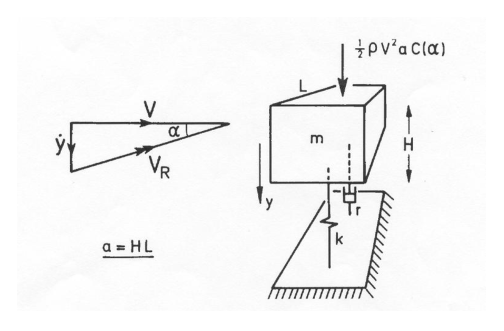
\includegraphics{img/ex2/galloping.eps}
\caption{}
\label{fig:ex2galloping}
\end{figure}

The forces that act on this element in the vertical direction are
\begin{itemize}
\item \textit{Inertia: $m\cdot \ddot{y}$}
\item \textit{Linear damping: $r\cdot\dot{y}$}
\item \textit{Elastic force: $k\cdot{y}$}
\item \textit{Driving force:} The wind relative to the prism $V_R$ is also shown in figure \ref{fig:ex2galloping}. Since the wind $V$ is purely horizontal, the vertical force due to $V_R$ will be a function of $\dot{y}$. For small $\alpha$ or equivalently large $V$, the angle $\alpha$ can be approximated by $\alpha=\frac{\dot{y}}{V}$ ($\sin{\theta}\approx \theta$ for small $\theta$). The force along the direction of the speed $\dot{y}$ is then given by
\begin{equation}
\frac{1}{2}\cdot\rho V^2aC(\alpha)
\end{equation}
where $C(\alpha)$ can be approximated by the 7th order polynomial
\begin{equation}\label{eqn:ex2calpha}
C(\alpha) = A_1\cdot \alpha-A_3 \cdot \alpha^3 + A_5\cdot \alpha^5 - A_7\cdot \alpha^7
\end{equation}
Met $\alpha$ expressed in radials, and the coefficiants $A_i$ as given in the assignment. This driving force can be seen as a nonlinear damping due to it being a function of $\dot{y}$
\end{itemize}
The full equations of the prism's motion are then given by
\begin{equation}\label{eqn:ex2model1line}
m\ddot{y}=-r\dot{y}-ky+\frac{1}{2}\rho V^2 a A_1 C(\alpha)
\end{equation}
\hfill\newline
Note that while the elastic force and the linear damping will counteract the accelaration, the driving force will increase it. When considering the system from now on the following values will be used
 \begin{equation}\label{eqn:ex2numericvalues}
m=1,\rho=1,r=1,k=100,a=1
\end{equation}

\subsection{A linear approximation}
First, the second order model equation (\ref{eqn:ex2model1line}) must be reduced to two first order equations
 \begin{align}
 \frac{dy}{dt}&=\dot{y}\label{eqn:dydt}\\
 \frac{d\dot{y}}{dt}&=-\frac{r}{m}\dot{y}-\frac{k}{m}y+\frac{1}{2m}\rho V^2 a A_1 C(\alpha)\label{eqn:ddotydt}
 \end{align}
 To find fixed points, $\frac{dy}{dt}$ as well as $\frac{d\dot{y}}{dt}$ must be zero. From the first condition it is found that $\dot{y}$ must be zero. This condition in (\ref{eqn:ddotydt}) then leads to $y=0$. So the origin is the only possible fixed point. In order to investigate it's stability, the system must be linearised. The only nonlinear term is the one containing $C(\alpha)$, which when linearising and evaluating in $0$ leads to $A_1$. The linearised system is then given by
 \begin{equation}
\begin{bmatrix}\frac{dy}{dt}\\\frac{d\dot{y}}{dt}\end{bmatrix}=\begin{bmatrix}0 & 1\\ -k & -r+\frac{1}{2}\rho VaA_1\end{bmatrix}\begin{bmatrix}y \\ \dot{y}\end{bmatrix}
\end{equation}
When using the values of \ref{eqn:ex2numericvalues} the Jacobian matrix and its trace and determinant become
\begin{equation}
J=\begin{bmatrix}0 & 1 \\-100 & -1+\frac{1}{2}VA_1\end{bmatrix}, \tau=-1+\frac{1}{2}VA_1, \Delta=100
\end{equation}
\hfill\newline
Since $\Delta$ is always positive, the fixed point will be a stable or unstable spiral  when $\tau<\sqrt{4\Delta}=20$. It's stability depends on $\tau$. When $V=V_C=\frac{2}{A_1}$, a bifurcation occurs when the real parts of the complex eigenvalues switch sign. When $V>V_C$, $\tau>0$ and the spiral is unstable. When $V<V_C$, $\tau<0$ and the spiral is stable. When only considering this linear model, the bifurcation that occurs is a degenerate Hopf bifurcation. When $V=V_C$ there will be a continuous band of closed orbits surrounding the origin.
\subsection{Simulating the system}
The system can be simulated using a SIMULINK model, shown in figure \ref{fig:ex1simmodel}. With this model the value of $V/V_c$ can be adapted during the simulation. The interpretations from the linearised model are checked with the full equations. When $V<V_C$, the fixed point is indeed stable. When increasing $V$ above $V_C$ however, a limit cycle appears. The fixed point at the origin is indeed an unstable spiral, but the appearance of the limit cycle points to a supercritical Hopf bifurcation instead of a degenerate Hopf bifurcation. This limit cycle can be explained when looking at (\ref{eqn:ex2calpha}), in the case $\alpha<1$. When $V>Vc$, this means that the coefficient of $\dot{y}$ in the driving force is greater then coefficient of $\dot{y}$ in the Linear damping when only considering the term $A_1\cdot \alpha$. This then leads to unstable behavior in every point of the $(y,\dot{y})$ plane. However, when also taking into account the term $-A_3\cdot \alpha^3$, the behavior will be stable for large values of $\alpha$ because the Driving force is weaker than the Linear damping. Thus, points very far from the origin are attracted towards it, and points near the origin are repelled from it. This explains the observed limit cycle.
\begin{figure}[htp]
\centering
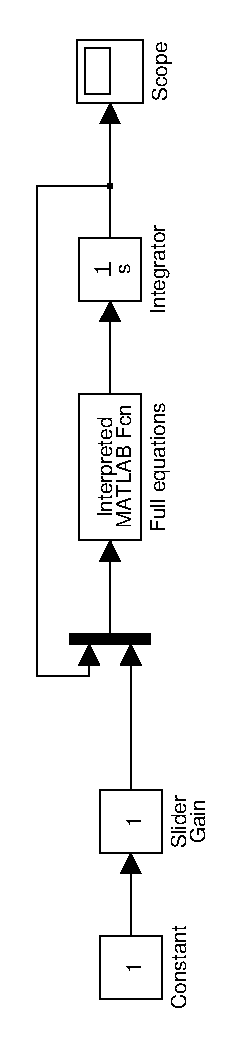
\includegraphics[angle=-90,trim= 0mm 7mm 5mm 10mm]{img/ex1/model1.eps}
\caption{}
\label{fig:ex1simmodel}
\end{figure}
\newline
When during the simulations $V$ is further increased, the radius of the limit cycle will suddenly jump to a distant value. When afterwards decreasing the $V$ again, the radius decreases continuously from the distant value, until it jumps again to a lower value. These two jumps are saddle-node bifurcations of cycles, as a stable and an unstable cycle collide and annihilate. Figure \ref{fig:ex227b} shows the evolution of the radius of the limit cycle for increasing $V$ on a step-by-step basis. The initial condition goes to zero, and when $V/V_C$ is increased, the two jumps in the amplitudes of the limit cycles become visible. Figure \ref{fig:ex227} at the end of this section shows a qualitative study in the $(y,\dot{y})$-space. In each subplot, the value of $V/V_C$ is increased by 0.2. The starting point of the simulation is denoted by a red dot. The simulation is carried out until a stable orbit is reached, which is shown in green. When $V/V_C$ is increased above 1, the first stable limit cycle appears. For increasing $V/V_C$, the radius of this limit cycle becomes wider and wider (Note that the axes are scaled so as to make the orbits appear circular).  When $V/V_C$ is increased above 1.8 to 2, the radius suddenly jumps to a distant value. When again decreasing $V/V_C$, the orbits steadily decrease from this value, until jumping back to the first stable limit cycle when $V/V_C$ is lowered below 1.4.  
\begin{figure}[htp]
\centering

\includegraphics{img/ex2/27b.eps}
\caption{}
\label{fig:ex227b}
\end{figure}

\subsection{Bifurcation diagrams}
From the previous section, it is clear that the system exhibits three bifurcations, of which the locations are approximately known from simulation.
\begin{itemize}
\item A supercritical Hopf bifurcation when $V/V_C$ = 1.
\item A saddle-node bifurcation of cycles when $V/V_C\in[1.2,1.4]$
\item A saddle-node bifurcation of cycles when $V/V_C\in[1.8,2]$
\end{itemize}
With the help of MATCONT, a continuation can be executed over the limit cycles. The result is shown in figure \ref{fig:ex2bifecht} as $A/V_C$ as a function of $V/V_C$, where $A$ is the maximal value of $y$ during a period. This figure confirms the previous analysis, as there is indeed a Hopf bifurcation at $V/V_C=1$, and two limit points of cycles at $V/V_C=1.241$ and$V/V_C=1.836$. The limit points of the cycles are thus well within the estimated bounds.
\newline
\newline As mentioned in the exercise session, the execution time for this continuation should be around 1 minute, in this case it was around 1.3 minutes. The execution time can be shortened by decreasing the number of mesh points or the increasing the minimum step size, but with a risk of missing one of the limit points of the cycles. Figure \ref{fig:bifA3d} shows the evolution of the limit cycles as a function of $V/V_C$. The cone folds into itself to form a region of $V/V_C$ where there are three limit cycles, of which the middle one is unstable. This was to be expected from figure \ref{fig:ex2bifecht}, which is just a cross section of figure \ref{fig:bifA3d}.
\begin{figure}[htp]
\centering

\includegraphics{img/ex2/bifA.eps}
\caption{}
\label{fig:ex2bifecht}
\end{figure}
\begin{figure}[htp]
\centering

\includegraphics{img/ex2/bifA3d.eps}
\caption{}
\label{fig:bifA3d}
\end{figure}

\begin{figure}[htp]
\centering

\includegraphics{img/ex2/27.eps}
\caption{}
\label{fig:ex227}
\end{figure}

\clearpage
\section{Predator-Prey Model}
\numberwithin{figure}{section}
\subsection{Introduction}
ALGEMENE ZEVER

The predator-prey model considered is
\begin{align}
\dot{x} &= x(x-0.2)(1-x) - xy \label{predmodelx} \\
\dot{y} &= xy-by-d \label{predmodely}
\end{align}
in which $b$ and $d$ are physical parameters. The predator dynamics are modeled by $y$ and the prey dynamics are modeled by $x$. The terms in the model each have an ecological interpretation:
\begin{itemize}
\item (\ref{predmodelx}) $x(x-0.2)(1-x)$: The growthfactor of the preys, independent of $y$.
\item (\ref{predmodelx}) $-xy$: The loss of preys, dependent on $y$. The more predators there are, the more preys will be lost.
\item (\ref{predmodely}) $xy$: The growthfactor of the predators, dependent on $x$. When there is more food, the predator population will grow faster.
\item (\ref{predmodely}) $-by$: Natural deaths of the predators.
\item (\ref{predmodely}) $-d$: A control parameter
\end{itemize}
In agreement with the ecological interpretation, only positive values of $x$ and $y$ are considered, unless specifically mentioned otherwise.

\subsection{A qualitative study for $d=0$}
In this section the control parameter $d$ is set to zero, and the parameter $b$ is considered in the region $b \in [0.2,1.5]$.
\subsubsection{The model without predators}
For an impression of the dynamics of the preys without predators, the model is considered for $y=0$. A number of simulations are carried out for initial values $x_0 \in [0,1.5]$. The results are shown in figure \ref{fig:ex3preyonly}. From this figure we can already see that there are 3 fixed points for $y=0$. There is a stable equilibrium for $x=1$, as denoted by the upper red curve. It's basin of attraction is $x_0 \in (0.2,+\infty]$. There is another stable equilibrium at population zero, denoted by the lower red curve, with a basin of attraction $x_0 \in [0, 0.2)$. The point $x=0.2$, denoted by the black curve, is an unstable equilibrium.

The interpretation is as follows: If the initial population is below a certain threshold, it will eventually go extinct. The threshold in this case is $0.2$. If the initial population is anywhere above this threshold, it will evolve to a constant population level 1.
\begin{figure}[htp]
\centering

\includegraphics{img/ex3/preyonly.eps}
\caption{}
\label{fig:ex3preyonly}
\end{figure}
\subsubsection{Steady state solutions and their stability}\label{sec:linearstab}
For the full model (\ref{predmodelx})-(\ref{predmodely}) to have steady state solutions, both $\dot{x}$ and $\dot{y}$ must be zero.
In the previous section we already found that there are three fixed points for $\dot{x}$ when $y$ is zero. As it turns out, $\dot{y}$ is zero too and the fixed points for the model without predators can be carried over to the full model. An additional fixed point is found for $(b,(b-0.2)(1-b))$, with a location dependent of $b$. 

In order to investigate the stability of these four fixed points, the Jacobian matrix $J(x,y)$ is considered as a function of $b$. The eigenvalues of $J$ will determine the stability, so this stability may be dependant on $b$. Note that we only consider $b \in [0.2,1.5]$. 
The Jacobian matrix is given by 
\begin{equation}
J(x,y) = \begin{bmatrix} (x-0.2)(1-x)+x(1-x)-x(x-0.2) & -x \\ y & x-b \end{bmatrix}
\end{equation}
\paragraph{Fixed point $(0,0)$}\hfill\newline
The Jacobian matrix at this point is given by 
\begin{equation}
J(x,y)|_{(0,0)}=\begin{bmatrix}
-0.2 & 0 \\
0 & -b
\end{bmatrix}
\end{equation}
It's eigenvalues are $\lambda_1-0.2$ and $\lambda_2-b$, with corresponding eigenvectors $v_1=(1,0)$ and $v_2=(0,1)$. When both eigenvalues are negative, this fixed point is a stable node. When $b$ is larger than $0.2$, $(1,0)$ will be the slower eigenvector. When $b$ is equal to $-0.2$ the fixed point is a stable star. The behavior of the fixed point is summarized in figure \ref{fig:ex300}.
\begin{figure}[H]
\centering
\subfloat[b=0.2]{
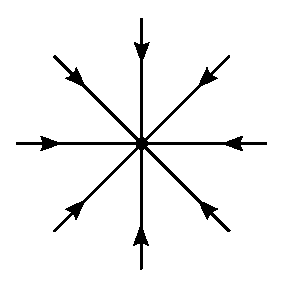
\includegraphics{img/stablestar.eps}}\hspace{18pt}
\subfloat[b>0.2]{

\includegraphics{img/stablenode.eps}}
\caption{}
\label{fig:ex300}
\end{figure}
\paragraph{Fixed point $(0.2,0)$}\hfill\newline
The Jacobian matrix at this point is given by 
\begin{equation}
J(x,y)|_{(0.2,0)}=\begin{bmatrix}
0.16 & -0.2 \\
0 & 0.2-b
\end{bmatrix}
\end{equation}
It's eigenvalues are $\lambda_1=0.16$ and $\lambda_2=0.2-b$, with corresponding eigenvectors $v_1=(1,0)$ and $v_2=(1/(5*(b - 1/25)),1)$. Since one of the eigenvalues is always positive, the fixed point will never be stable. When $b=0.2$, one of the eigenvalues is zero, and the stability cannot be derived from the linearization. A detailed analysis with PPLANE reveals that it is in fact a saddle node, with the stable and unstable manifold determined by the eigenvectors. When $b>0.2$, the fixed point is still a saddle point with unstable manifold $v_1$ and stable manifold $v_2$. The behavior of the fixed point is summarized in figure \ref{fig:ex3020}.
\begin{figure}[H]
\centering
\subfloat[b>=0.2]{
\includegraphics{img/saddle020.eps}}
\caption{}
\label{fig:ex3020}
\end{figure}
\paragraph{Fixed point $(1,0)$}\hfill\newline
The Jacobian matrix at this point is given by 
\begin{equation}
J(x,y)|_{(0.2,0)}=\begin{bmatrix}
-0.8 & -1 \\
0 & 1-b
\end{bmatrix}
\end{equation}
It's eigenvalues are $\lambda_1=-0.8$ and $\lambda_2=1-b$, with corresponding eigenvectors $v_1=(1.8-b,1)$ and $v_2=(0,1)$. When $b \in [0.2,1)$, the eigenvalues have opposite signs and the fixed point is a saddle node with stable manifold $v_1$ and unstable manifold $v_2$. When $b$ equals 1 another borderline case occurs. One of the eigenvalues is zero and the linearization cannot determine the stability.  As detailed analysis with PPLANE shows this fixed point is in fact half-stable, as it undergoes a transcritical bifurcation. When $b \in [1,1.5]$ both eigenvalues are negative and the fixed point is a stable node, with slow eigendirection $v_2$.The behavior of the fixed point is summarized in figure \ref{fig:ex310}.
\begin{figure}[H]
\centering
\subfloat[$b \in [0.2, 1)$]{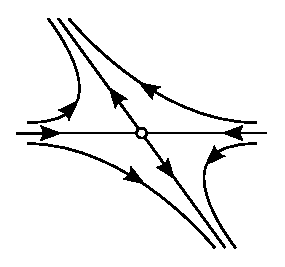
\includegraphics{img/saddle011.eps}}\hspace{18pt}
\subfloat[$b = 1$]{
\includegraphics{img/saddle10.eps}}\hspace{18pt}
\subfloat[$b \in (1,1.5)$]{
\includegraphics{img/saddle012.eps}}
\caption{}
\label{fig:ex310}
\end{figure}

\paragraph{Fixed point $(b,(b-0.2)(1-b))$}\hfill\newline
The Jacobian matrix at this point is given by 
\begin{equation}
J(x,y)|_{(b,(b-0.2)(1-b))}=\begin{bmatrix}
-2b^2+1.2b & -b \\
(1-b)(b-0.2) & 0
\end{bmatrix}
\end{equation}
Its eigenvalues are less straightforward to compute. They are given by the roots of the quadratic equation 
\begin{equation}
\lambda^2-b(1.2-2b)\lambda+b(1-b)(b-02.)
\end{equation}
The discriminant of this quadratic equation is a function of $b$, and as is mentioned in the assignment has zeros at $b=-.9318$, $b=0$, $b=0.240923$ and $b=0.890889$. The discriminant will change it's sign on every zero, and this will determine wether the eigenvalues have a nonzero imaginary part. A plot of the real and imaginary parts of $\lambda_1$ and $\lambda_2$ is shown in figure \ref{fig:ex3eigvalues}. A plot of the trace and the determinant is shown in figure \ref{fig:ex3tracedeterminant}. As can be seen in figure \ref{fig:ex3eigvalues}, the imaginary parts indeed appear and disappear at the zeros of the discriminant. Furthermore, it is seen that the real parts of the eigenvalues pass through zero several times, so there will be changes in stability.
\begin{figure}[htp]
\centering

\includegraphics{img/ex3/eigvalues.eps}
\caption{}
\label{fig:ex3eigvalues}
\end{figure}
\begin{figure}[htp]
\centering

\includegraphics{img/ex3/tracedeterminant.eps}
\caption{}
\label{fig:ex3tracedeterminant}
\end{figure}
\newline An overview of the changes in topology are given for meaningful values of $b$, again in the interval $b\in[0.2 1.5]$
\begin{description}
\item[$b = 0.2$]\hfill\newline At this point, $Re(\lambda_2)$ changes from negative to positive, so the fixed point has two positive eigenvalues and becomes an unstable node.
\item[$b \in (0.2,0.240923)$]\hfill\newline In this region the fixed point is an unstable node.
\item[$b = 0.240923$]\hfill\newline At this point the eigenvalues of $J$ become imaginary, and the unstable node will bend into an unstable spiral. This is not a bifurcation since the topology is not structurally different. This point is called a degenerate source.
\item[$b \in (0.240923,0.6)$]\hfill\newline In this region the fixed point is an unstable spiral.
\item[$b= 0.6$]\hfill\newline At this point $Re(\lambda_{1,2})$ will turn negative. This is a sign of a Hopf bifurcation (possibly degenerate), and it marks the change from an unstable to a stable spiral.
\item[$b \in (0.6, 0.890889)$]\hfill\newline In this region the fixed point is a stable spiral.
\item[$b = 0.890889$]\hfill\newline At this point $Im(\lambda_{1,2})$ become zero again and the stable spiral becomes a stable node.
\item[$b \in (0.8890889,1)$]\hfill\newline In this region the fixed point is a stable node.
\item[$b=1$]\hfill\newline At this point $Re(\lambda_2)$ will change from negative to positive so $\lambda_1$ and $\lambda_2$ have opposite signs. The stable node will turn into a saddle point. This point engages in a transcritical bifurcation with the fixed point $(1,0)$.
\item[$b\in(1,1.5)$]\hfill\newline In this region the fixed point is a saddle point. 
\end{description}
An overview of the diferent topologies is given in figure \ref{fig:ex3bb}. An overview of the trajectory of this fixed point in function of $b$ is given in figure \ref{fig:ex3trajectory}. This figure shows that for $b=0.2$ and $b=1$ this fixed point will indeed interact with other fixed points, as was seen in the transcritical bifurcation at $b=1$.
\begin{figure}[htp]
\centering
\subfloat[$b \in (0.2,0.240923)$]{
\includegraphics{img/unstablenode.eps}}\hspace{18pt}
\subfloat[$b \in (0.240923,0.6)$]{
\includegraphics{img/unstablespiral.eps}}\hspace{18pt}
\subfloat[$b \in (0.6, 0.890889)$]{
\includegraphics{img/stablespiral.eps}}\\
\subfloat[$b \in (0.8890889,1)$]{
\includegraphics{img/saddle012.eps}}\hspace{18pt}
\subfloat[$b=1$]{
\includegraphics{img/saddle10.eps}}\hspace{18pt}
\subfloat[$b\in(1,1.5)$]{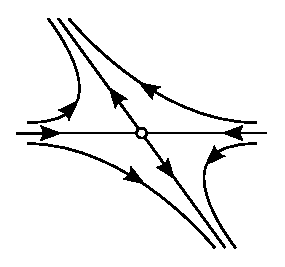
\includegraphics{img/saddle011.eps}}
\caption{}
\label{fig:ex3bb}
\end{figure}
\begin{figure}[htp]
\centering

\includegraphics{img/ex3/btrajectory.eps}
\caption{}
\label{fig:ex3trajectory}
\end{figure}

In order to verify the analysis, some phase diagrams generated with PPLANE are shown in figures \ref{fig:PPLANE1} to \ref{fig:PPLANE5}, for different values of $b$. For increased readability of this report, the diagrams are in appendix.

\subsubsection{Separatrices and regions of attraction}
In order to find the separatrices we must find the boundaries between regions of attraction and regions of repulsion. Two different values for $b$ are considered, namely $b=0.5$ and $b=0.65$. 

When $b=0.5$ the phase diagram can be seen in figure \ref{fig:PPLANE1}. Since the spiral is unstable, every initial point with $y>0$ will converge to the stable node at the origin. When $y<0$, there is a boundary between a stable and an unstable region, determined by the stable manifold of the saddle node at $(0.2,0)$. In order to calculate these boundaries, the stable manifold must be simulated backwards from the saddle node. Two problems arise when doing this:
\begin{itemize}
\item The simulation must go backwards. To this end the signs of the derivatives in the model equations (\ref{predmodelx})-(\ref{predmodely}) are flipped. This way the simulation will go backwards in time.
\item The simulation should start on the stable manifold, as close as possible to the saddle point. The initial points are chosen as a small perturbation from the saddle point along the direction of the stable manifold computed in the linearized analysis.
\end{itemize}
The separatrices and regions of attraction for $b=0.5$, along with the stable manifold of the saddle, are shown in figure \ref{fig:ex3separatrices1}.

When $b=0.65$ the phase diagram is shown in figure \ref{fig:PPLANE3}. The spiral has now become stable, and there will be two regions of attraction, one for the stable node at the origin and one for the spiral. The situation for $y<0$ remains the same. The calculations are executed similar to the case $b=0.5$, and the results are shown in figure \ref{fig:ex3separatrices2}
\begin{figure}[htp]
\centering
\subfloat[$b=0.5$]{
\includegraphics{img/ex3/separatrices1.eps}\label{fig:ex3separatrices1}}
\subfloat[$b=0.65$]{
\includegraphics{img/ex3/separatrices2.eps}\label{fig:ex3separatrices2}}
\caption{}
\label{fig:}
\end{figure}
\subsubsection{An overview of the changes in the phase diagram}
A lot of information regarding the stability of the fixed points was already given in section \ref{sec:linearstab}. This section will summarize these results in a qualitative overview of the changes in the phase diagram for varying $b$. More attention will also be given to the bifurcations occuring.

\subsubsection{An important global bifurcation}
As established in the previous section, a supercritical Hopf bifurcation occurs at $b=0.6$. What is not yet established is where the stable limit cycle needed for this bifurcation comes from. A detailed analysis of the phase diagrams for $b \in [0.52 0.57]$ reveals the bifurcation from which the stable limit cycle originates. A help to understanding this bifurcation is the behavior of the stable manifold of the saddle at $(0.2,0)$. When $b<b_{crit}$, the stable manifold will disappear into the unstable spiral.When $b>b_{crit}$, the stable manifold goes off to $+\infty$.  When $b=b_{crit}$, the stable manifold of the saddle point will be connected to the unstable manifold of the saddle point at $(1,0)$ through a heteroclinic trajectory.The evolution of the stable manifold is shown in figure \ref{fig:ex3unstablemanfold}.
\newline
\newline
When $b>b_{crit}$ the heteroclinic trajectory detaches from the saddle points and constitutes a stable limit cycle. In agreement with Strogatz' definition of a homoclinic bifurcation of cycles this can be called a heteroclinic bifurcation of cycles. The stable limit cycle will shrink with increasing $b$, as shown in figure \ref{fig:ex3homoclinicorbits}, until it collapses onto the fixed point for the Hopf bifurcation.
\newline
\newline
Through iterative simulation of the stable manifold it is found that it forms a heteroclinic trajectory at $b\approx0.538$. The phase diagram is shown in figure \ref{fig:PPLANEhomoclinic}.
\begin{figure}[htp]
\centering
\subfloat[unstable manifold]{
\includegraphics{img/ex3/homoclinicmanfold.eps}\label{fig:ex3unstablemanfold}}\hspace{18pt}
\subfloat[limit cycles]{
\includegraphics{img/ex3/homoclinicorbits.eps}\label{fig:ex3homoclinicorbits}}
\caption{}
\label{fig:}
\end{figure}
The period of the limit cycles is very long just after the heteroclinic bifurcation, and becomes shorter and shorter moving towards the Hopf bifurcation. This is because the heteroclinic bifurcation resembles an infinite period bifurcation in the sense that the initial heteroclinic trajectory has an infinite period. The period length for increasing $b$ is shown in Table \ref{tbl:orbitperiod}.  The decreasing of the period is clearly visible. The table shows the results computed with PPLANE, but the accuracy of these results is not known.
\begin{table}[H]
\begin{center}
\begin{tabular}{|l|c|}
  \hline                        
  $b$ & Period(s) \\
  \hline 
  $b_{crit}$ & $\infty$ \\
  0.55 & 35.5 \\
  0.56 & 29.6 \\
  0.57 & 26.1 \\
  0.58 & 23.7 \\
  0.59 & 21.8 \\
  \hline  
\end{tabular}
\end{center}
\caption{}
\label{tbl:orbitperiod}
\end{table}
\begin{figure}[htp]
\centering

\includegraphics{img/ex3/PPLANEhomoclinic.eps}
\caption{}
\label{fig:PPLANEhomoclinic}
\end{figure}
\subsubsection{Evolution of $x$ and $y$ on the limit cycles}
In this section we compare the behavior of the populations $x$ and $y$ on a limit cycle. We compare a limit cycle for $b=0.545$, close to the heteroclinic cycle, and a limit cycle for $b=0.59$ corresponding to an almost harmonic oscillation. The distance between points on the limit cycle for regular time intervals is shown in figure \ref{fig:ex3speeds}. From these distances the speed at a point on the limit cycle can be calculated. In figure \ref{fig:ex3coloredorbits} both limit cycles are shown with a coloration depending on the speed, red being fast and blue being slow. As could already be seen from figure \ref{fig:ex3speeds}, the speed levels out for $b=0.59$.
\begin{figure}[htp]
\centering

\includegraphics{img/ex3/speeds.eps}
\caption{}
\label{fig:ex3speeds}
\end{figure}
\begin{figure}[htp]
\centering

\includegraphics{img/ex3/coloredorbits.eps}
\caption{}
\label{fig:ex3coloredorbits}
\end{figure}
\subsection{Bifurcation analysis}
In this section, the complete bifurcation diagram will be computed with MATCONT, for $b \in[0.1,0.5]$.
\subsubsection{Case $d=0$}
The bifurcation diagram for $d=0$ is shown in figure \ref{fig:ex3bif} for $x$ vs $b$ and $y$ vs $b$. UITLEG OVER BIFURCATIES

The limit cycles computed with MATCONT are shown in figure \ref{fig:ex3dlimitcycles}. This figure indeed shows the heteroclinic bifurcation, with the radius of the limit cycle decreasing until it vanishes in a Hopf bifurcation. 
\begin{figure}[htp]
\centering
\subfloat[$x$ vs $b$]{\includegraphics{img/ex3/bifx.eps}}
\subfloat[$y$ vs $b$]{\includegraphics{img/ex3/bify.eps}}
\caption{}
\label{fig:ex3bif}
\end{figure}
\begin{figure}[htp]
\centering
\includegraphics{img/ex3/3dlimitcycles.eps}
\caption{}
\label{fig:}
\end{figure}


\subsubsection{Case $d\ne0$}
\begin{figure}[htp]
\centering
\subfloat[$x$ vs $b$]{\includegraphics{img/ex3/bifposx.eps}}
\subfloat[$y$ vs $b$]{\includegraphics{img/ex3/bifposy.eps}}
\caption{}
\label{fig:ex3bifpos}
\end{figure}
\begin{figure}[htp]
\centering
\subfloat[$x$ vs $b$]{\includegraphics{img/ex3/bifnegx.eps}}
\subfloat[$y$ vs $b$]{\includegraphics{img/ex3/bifnegy.eps}}
\caption{}
\label{fig:ex3bifpos}
\end{figure}














\clearpage
\section{Lyapunov's exponents, Chua's circuit and Duffing oscillator with periodic forcing}
In this section, different systems all related to chaos in the phase plane are studied. In a first subsection, the importance of Lyapunov exponents in dynamical systems will be explained, as well as the numerical computations required to obtain them. In a second subsection the Duffing oscillator with periodic forcing is studied and simulated, to show chaotic behavior. The oscillator will also be brought in the subharmonic regime, to show its difference from the chaotic case. In a last subsection Chua's circuit will be studied, an electrical circuit known to exhibit chaotic behavior. 
\subsection{Lyapunov exponents of the Lorenz Equations}
The Lyapunov exponents for an attractor of a dynamical system are defined as follows. Consider the evolution of an infinitesimal sphere of perturbed initial conditions. During its evolution, the sphere will become distorted into an infinitesimal ellipsoid. When the length of the $k$th principal axis of the ellipsoid is denoted by $\delta_k(t)$, it's length will evolve according to $\delta_k(t)~\delta_k(0)e^{\lambda_kt}$. The $\lambda_k$ are the Lyapunov exponents. For the remainder of the discussion, the Lyapunov exponents will be assumed to be ordered, with $\lambda_1\geq\lambda_2\geq...$. For large $t$, the diameter of the ellipsoid is controlled by the most positive component $v_1$ corresponding to $\lambda_1$. Different types of attractors discern themselves through this largest Lyapunov exponent.
\begin{description}
\item[Stable fixed point] For a set of perturbed initial conditions in the region of attraction, they will all end up in the same point. Every axis of the ellipsoid collapses to zero, and all the Lyapunov exponents are negative.
\item[Stable limit cycle] When a set of perturbed initial conditions is attracted towards the limit cycle, their distance will be constant when they have reached the limit cycle. This is because they will travel on the limit cycle, all with exactly the same period. Therefore the largest Lyapunov exponent must be zero.
\item[Chaotic/strange attractor] The definition of these attractors states that they have \textit{"sensitive dependence on initial conditions"}. This means that the distance between infinitesimally close initial conditions will grow, instead of evolving to zero or remaining constant. Therefore, the largest Lyapunov exponent must be positive.
\end{description}

The Lyapunov exponents can be computed numerically, as explained in the lectures. The difficulty lies in the fact that almost any initial disturbance will have a component along $v_1$. As explained before when the system is chaotic this component will be enormously amplified relative to the other components. When iterating multiple displacements they will all become almost parallel, and the other Lyapunov exponents are hard to extract. This problem is solved by frequently reorthogonalizing the vectors, as in the MATLAB function \code{lyapunov.m}. This function takes 4 arguments: the differential equations describing the system, the number of iterations $kmax$, the timestep $st$ to be taken for simulation every iteration, the initial phase point $x$ and an ODE solver. The procedure is as follows:
\begin{itemize}
\item The initial tangent vectors are taken to be the identity matrix $I$. It's evolution will be modeled by the linearised system at the phase point. This can be done by multiplying with the Jacobian matrix, a computation that is in \code{rhs\_lorenz.m}. The Jacobian for the Lorenz equations is
\begin{equation}
\begin{bmatrix} -\sigma&  \sigma   & 0\\
 (r-z)  &  -1  &   -x \\
  y  &     x &    -b\end{bmatrix}
\end{equation}
\item In every iteration $j=1,..,kmax$
\begin{itemize}
\item The evolution of the phase point is integrated over $st$ along with the tangent vectors.
\item The tangent vectors are orthogonalised via Gramm-Schmidt orthogonalization.
\item The evolution of the length of the $i$th largest vector is used to update the approximation of the $i$th largest Lyapunov exponent. 
\item The vectors are normalized
\end{itemize}
\item The Lyapunov exponents are returned as the last updated approximation.
\end{itemize}
Figure \ref{fig:ex4lyapunovlorenz} shows the results when this method is applied to the Lorenz equations. When suitable parameters are chosen, the function returns are a good approximation
\begin{equation}
\lambda_1=0.8788\mbox{\hspace{6pt}}(0.9),\mbox{\hspace{12pt}} \lambda_2= -0.0017 \mbox{\hspace{6pt}}(0),\mbox{\hspace{12pt}} \lambda_3= -14.5407 \mbox{\hspace{6pt}}(-14.57)
\end{equation}
The influence of the parameters is rather straightforward. The experiments are carried out for varying $st$ and $kkmax$ when keeping the other parameters constant. Care is taken that the product of $st$ and $kkmax$ stays constant, so that the calculations all take equal simulated time. The result is shown in figure \ref{fig:ex4comparison}. When increasing $kkmax$, the solutions will have stabilised more, and the error decreases. When increasing $st$, the approximation gets coarser, and the errors grow.
\begin{figure}[htp]
\centering
\includegraphics{img/ex4/lyaplorenz.eps}
\caption{The approximations for the Lyapunov exponents as a function of time. The parameters used are $x=[0.5,0.5,0.5],kmax=8000,st=0.05$.}
\label{fig:ex4lyapunovlorenz}
\end{figure}
\begin{figure}[H]
\centering
\subfloat[kkmax]{\includegraphics{img/ex4/lyapkkmax.eps}}
\subfloat[st]{\includegraphics{img/ex4/lyapst.eps}}
\caption{}
\label{fig:ex4comparison}
\end{figure}
\subsection{the Duffing oscillator with periodic forcing}
The Duffing oscillator with periodic forcing is described by the following equation 
\begin{equation}
\ddot{x}+k\dot{x}+x^3=B\cos{t}.
\end{equation}
The long term behavior of the system depends on the parameters $B$ and $k$, and the different possible regimes are shown in appendix as figure \ref{fig:ex4duffingscheme}. First the system will be studied in the chaotic region. Therefore the parameters are chosen to be $B=11$ and $k=0.15$. The result of a first simulation is shown in figure \ref{fig:ex4duffingexample}, where indeed the trajectory does not seem to converge to a limit cycle or stable point. To show that it is indeed chaotic, the behavior of two close initial points is simulated in figure \ref{fig:duffingchaoticposition}. The figures show the behavior of the two points at times between 75 and 90. This time interval is chosen to visually illustrate the chaotic behavior. In interval 1, the two trajectories are practically indescernable. In interval 2 and 3 the trajectories start to slowly diverge, and in interval 4 the trajectories are no longer close so that in interval 5 and 6 they show completely different behavior. A plot of $x$ and $\dot{x}$ in function of the time is shown in figure \ref{fig:duffingtime} and \ref{fig:duffingtimeb}. These figures illustrate that the trajectories that are almost identical up until 75, are rapidly exhibiting completely different behavior in just a few seconds.
\begin{figure}[htp]
\centering
\includegraphics{img/ex4/duffingexample.eps}
\caption{}
\label{fig:ex4duffingexample}
\end{figure}
\begin{figure}[htp]
\centering
\includegraphics{img/ex4/duffingchaoticposition.eps}
\caption{}
\label{fig:duffingchaoticposition}
\end{figure}
\begin{figure}[htp]
\centering
\subfloat{\includegraphics{img/ex4/duffingchaotictimea.eps}\label{fig:duffingtime}}\\
\subfloat{\includegraphics{img/ex4/duffingchaotictimeb.eps}\label{fig:duffingtimeb}}
\caption{}
\label{fig:}
\end{figure}



\clearpage
\section{Pattern formation}\label{sec:patternformation}
In this section the Brusselator model is studied, which is a system of two interacting species. This model is of interest because it exhibits Turing patterns. 
\newline
\newline
First the equations will be studied for a one-dimensional spatial domain. For this one-dimensional case the conditions for Turing instability will be studied. 
\newline
\newline
Later on a simulator will be used to study the two-dimensional case, and some of the results for the one-dimensional case will be reused.
\subsection{The Brusselator model}
The equations for the one-dimensional case are given by
\begin{align}
u_t&=D_uu_{xx}+A-(B+1)u+u^2v \label{eqn:brusu}\\ 
v_t&=D_vv_{xx}+Bu-u^2v \label{eqn:brusv}
\end{align}
where $D_u$ and $D_v$ are the diffusion constants of the two species $u$ and $v$, and $A$ and $B$ are concentrations which are kept constant. This system has a spatially uniform steady state, in which $u_0=A$, $v_0=B/A$. The equations (\ref{eqn:brusu})-(\ref{eqn:brusv}) contain a diffusion term dependent on $u_{xx}$ or $v_{xx}$ and form a PDE system. The equations without this diffusion terms 
\begin{align}
u_t&=A-(B+1)u+u^2v \label{eqn:brusuode}\\ 
v_t&=Bu-u^2v \label{eqn:brusvode}
\end{align}
form an ODE system that will also be studied. 
\subsection{One-dimensional case}
In this section some properties such as the onset of Turing instability will be derived for the one-dimensional case.
\subsubsection{Stability of the spatially uniform steady state}
In order to study the stability of $u_0=A$, $v_0=B/A$, the model is linearised around this state.  To this end the derivative is taken with respect to $u$ and $v$.
\begin{equation}\label{eqn:linbrusselator}
\begin{bmatrix}u_t \\ v_t \end{bmatrix}=\begin{bmatrix}D_uu_{xx}\\ D_vv_{xx}\end{bmatrix}+\begin{bmatrix}-(B+1)+2uv & u^2 \\
B-2uv & -u^2 \end{bmatrix}\begin{bmatrix}u\\v\end{bmatrix}
\end{equation}
And after filling in $u_0=A$, $v_0=B/A$
\begin{equation}
\begin{bmatrix}u_t \\ v_t \end{bmatrix}=\begin{bmatrix}D_uu_{xx}\\ D_vv_{xx}\end{bmatrix}+\begin{bmatrix}B-1 & A^2 \\
-B & -A^2 \end{bmatrix}\begin{bmatrix}u\\v\end{bmatrix}
\end{equation}
\newline
\newline
The linear evolution matrix of a Fourier mode $(u_F,v_F) = (u_1,v_1)exp(\lambda t + ikx)$ can then easily be found by noting that $u_{xx}$ and $v_{xx}$ simply become $-k^2(u_F,v_F)$. Filling in the Fourier mode and its spatial derivatives in (\ref{eqn:linbrusselator}) results in a linear evolution matrix given by
\begin{equation}\label{eqn:linevmat}
\begin{bmatrix}(B-1)-D_uk^2 & A^2 \\ -B & -A-D_vk^2\end{bmatrix}
\end{equation}
\paragraph{Eigenvalues of the linear evolution matrix}\hfill\newline
The eigenvalues of the linear evolution matrix given by (\ref{eqn:linevmat}) can be computed in a straightforward fashion. The trace of this matrix equals
\begin{equation}
\Sigma=B-1-A^2-k^2(D_u+D_v)
\end{equation} 
and it's determinant equals
\begin{equation}
\Delta = A^2 + k^2(A^2D_u+(1-B)D_v)+k^4D_uD_v.
\end{equation}
The eigenvalues are then the solutions of the characteristic equation, given by
\begin{equation}
s_{\pm}=\frac{1}{2}(\Sigma\pm\sqrt{\Sigma^2-4\Delta}),
\end{equation}
also called a \textit{dispersion relation}.

\subsubsection{The onset of Turing instability}
When explicitly writing the eigenvalues as a real and imaginary part $s_{\pm}=\sigma\pm i\omega$, a Turing instability occurs when $\sigma$ changes sign, and $\omega$ is zero. This can be explained as follows. The Turing instability occurs when the solution of the ODE system is stable and the solution of the PDE system is unstable. VERDER OVER NADENKEN
\paragraph{The critical value $B_T$}\hfill\newline
For $B$ very small, the spatially uniform solution is stable. This can be seen because the trace is negative, and the determinant is positive, so the eigenvalues will have negative real parts. When increasing $B$ at a given point Turing instability will set in. This critical value $B_T$ can be computed as follows. Turing instability can start for one of two reasons.
The Jacobian of the ODE system $J_O$ has trace$<0$ and determinant$>0$ (stable region) and either
\begin{itemize}
\item The Jacobian of the PDE system $J_P$ has trace$>0$ and determinant$>0$ (unstable region)
\item The Jacobian of the PDE system $J_P$ has determinant$<0$ (saddle region)
\end{itemize}
The first possibility is quickly ruled out because the $trace(J_p)$ is simple $trace(J_O)-k^2(D_u+D_v)$. since the diffusion coefficients are positive numbers, $trace(J_p)$ will never be positive while $trace(J_O)$ is negative.
\newline
\newline
The second possibility implies that the determinant should be negative. The instability will thus start when the determinant is negative. Setting the determinant to zero  with constant $A$, $D_u$ and $D_v$ gives an equation in two variables $B$ and $k$.
\begin{align}
\Delta = 0 &=A^2 + k^2(A^2D_u+(1-B)D_v)+k^4D_uD_v \\
B&=A^2\frac{D_u}{D_v}+1+\frac{A^2}{k^2D_v}+k^2D_u  \label{eqn:bfunck}
\end{align}
$B$ can now be seen as a function of $k$. To solve the equation it must be noted that the instability will start for a critical wavenumber $k_T$ for which the corresponding $B$ is the lowest. This critical wavenumber is the minimum of $B(k)$ and can be computed by setting the derivative to $k$ to zero.
\begin{align}
\frac{\delta B}{\delta k}=0&=2kD_u-2\frac{A^2}{D_vk^3} \\
k_T&=\left(\frac{A^2}{D_uD_v}\right)^{\frac{1}{4}}
\end{align}

By filling in this value in (\ref{eqn:bfunck}) the critical value $B_T$ can be found
\begin{align}
B_T&=A^2\frac{D_u}{D_v}+1+\frac{A^2}{A\sqrt{\frac{D_v}{D_u}}}+A\sqrt{\frac{D_u}{D_v}} \\
 &=(1+A\eta)^2
\end{align}
with 
\begin{equation}
\eta=\sqrt{D_u/D_v}
\end{equation}
\subsubsection{Instability in the ODE system}
When considering the ODE system (\ref{brusuode})-(\ref{brusvode}) with jacobian matrix given by
\begin{equation}
J_O=\begin{bmatrix}(B-1) & A^2 \\ -B & -A^2\end{bmatrix},
\end{equation}
it is easily seen that the system exhibits a Hopf biforcation when $B_H=1+A^2$. The determinant $A^2$ is always positive, and when $B_H=1+A^2$, the trace changes sign, thus altering the stability of the spiral. This Hopf bifurcation might occur for a lower value of $B$ than the Turing instability, the latter being dependant on the parameter $\eta$. The critical value $\eta_T$ can be computed as follows
\begin{align}
1+A^2&=(1+A\eta_T)^2 \\
\eta_T&=\frac{\sqrt{A^2+1}-1}{A}
\end{align}
The Turing stability sets in first when $\eta<\eta_T$.
\subsection{Two-dimensional case: Brusselator applet}






\clearpage
\appendix
\section{PPLANE Figures}
\numberwithin{figure}{section}
\begin{figure}[htp]
\centering
\includegraphics{img/ex3/PPLANE1.eps}
\caption{}
\label{fig:PPLANE1}
\end{figure}
\begin{figure}[H]
\centering
\includegraphics{img/ex3/PPLANE2.eps}
\caption{}
\label{fig:}
\end{figure}
\begin{figure}[htp]
\centering
\includegraphics{img/ex3/PPLANE3.eps}
\caption{}
\label{fig:PPLANE3}
\end{figure}
\begin{figure}[htp]
\centering
\includegraphics{img/ex3/PPLANE4.eps}
\caption{}
\label{fig:}
\end{figure}
\begin{figure}[htp]
\centering
\includegraphics{img/ex3/PPLANE5.eps}
\caption{}
\label{fig:PPLANE5}
\end{figure}
\clearpage
\section{Duffing regimes}
\begin{figure}[htp]
\centering
\includegraphics[scale=1.5]{img/ex4/duffingscheme.eps}
\caption{}
\label{fig:ex4duffingscheme}
\end{figure}



\end{document}



%%% Local Variables: 
%%% mode: latex
%%% TeX-master: t
%%% End: